\documentclass[12pt,twoside]{book}


\usepackage[thesis]{parsa}
\usepackage{xepersian}

\settextfont{XB Niloofar}


% --- Institute's Information
\InstituteLogo{BNUT-Logo}{BNUT-Logo}[35mm][35mm]
\Institute{دانشگاه صنعتی نوشیروانی بابل}{Babol Noshirvani University of Technology}
\Faculty{دانشکده برق و کامپیوتر}{Faculty of Computer Science}


% --- Student's Information
\StudentName{محمدعلی علی پناه}{Mohammad ali Ali panah}
\StudentMajor{کامپیوتر}{Computer}
\StudentDegree{کارشناسی‌}{Bachelor}
\StudentNumber{983212051}


% --- Thesis/Dissertation's Information
\ParsaTitle{سامانه اجراي كد از راه دور}{Remote code execution engine}
\ParsaCompilationDate{شهریور ۱۴۰۲}{August, 2023}


% --- Supervisor's Information
\SupervisorName{دکتر غلامی}{Dr.Gholami} 

\begin{document}
\renewcommand{\contentsname}{فهرست مطالب}
\renewcommand{\listfigurename}{فهرست شکل‌ها}
\renewcommand{\bibname}{مراجع}

%------------------------------------------------------------------------
%	FRONT MATTER
%------------------------------------------------------------------------
\frontmatter \pagestyle{empty}
\pagenumbering{adadi}

% Titlepage in Persian
\titlepageParsi
\cleardoublepage

% A picture for IN THE NAME OF GOD
\ParsaPicture{0-Front-Matter/In-The-Name-of-Allah.png}
\clearpage

% Dedication
\begin{center}
    \section*{تقدیم}
\end{center}
این صفحه برای تقدیم اثر از سوی دانشجو به افراد یا سازمان‌هایی که برای او مهم هستند در نظر گرفته شده است؛ در غیر این‌صورت، این صفحه را پاک کنید.
\clearpage


\pagenumbering{harfi} \pagestyle{plain}

\begin{ParsaAbstractParsi}
    محتویات چکیده شامل سه بخش مقدمه¬ای کوتاه و بیان مسأله، روش تحقیق و ویژگی¬های آن و نهایتا نتایج تحقیق و کاربردها (در صورت لزوم) باشد. در متن چکیده، از ارجاع به منابع و اشاره به جدول‌ها و نمودارها اجتناب شود. در صورت نیاز به معرفی حوزه تحقیق و مبانی تئوری آن، حداکثر در پاراگراف اول چکیده مطرح گردد. فقط به ارائهی روش تحقیق و نتایج نهایی و محوری بسنده کرده و از ارائهی موضوعات و نتایج كلی اجتناب شود. كلمات یا عباراتی كه در این بخش توضیح داده می‌شود، باید كاملاً محوری و مرتبط با موضوع تحقیق باشند. متن چکیده حداکثر یک صفحه باشد. جمله اول چکیده بیان‌کننده هدف نهایی از انجام پژوهش است. جملات بعدی به منظور توضیح پیرامون هدف اصلی آورده می‌شوند. سپس، روش‌هایی که برای انجام پروژه مورد استفاده قرار خواهند گرفت به طور خلاصه و کلی مورد اشاره قرار می‌گیرند. در نهایت، نتایج مورد انتظار، نوآوری‌ها و کاربردهای این پژوهش عنوان می‌گردند. در چكیده از ارجاع به منابع، ذكر روابط ریاضی و بیان تاریخچه خودداری ‌می‌شود.
    از زیرنویس کلمات مخفف شده در چکیده خودداری شود. کلمات مخفف شده در لیست کلمات اختصاری قابل مشاهده است.


    \bigskip\noindent
    \متن‌سیاه{کلمات کلیدی:} تعداد كلمات یا عبارات كلیدی حداكثر می‌تواند هفت كلمه یا عبارت باشد که با نقطه ویرگول (؛) از یک‌دیگر جدا شده‌اند. مانند: سختی؛ تنش؛ عملکرد
\end{ParsaAbstractParsi}
\clearpage

\tableofcontents
\listoffigures


%------------------------------------------------------------------------
%	MAIN MATTER
%------------------------------------------------------------------------
\mainmatter \pagestyle{parsaheadings}

\chapter{آشنایی با پژوهش}

\chapter{مفاهیم پایه}

در این فصل به معرفی تکنولوژی و فریمورک های به کار رفته در پروژه میپردازیم.

\section{Firecracker}
در قلب پروژه Firecracker قرار دارد. Firecracker یک مانیتور ماشین مجازی است که از KVM استفاده می‌کند و
وظیفه اش ساخت و مدیریت ماشین های مجازی است.
Firecracker توسط تیم وب سرویس آمازون توسعه داده شده و در پروژه Fargate و Lambda این شرکت نیز استفاده شده است.

\begin{figure}[h]
    \centering
    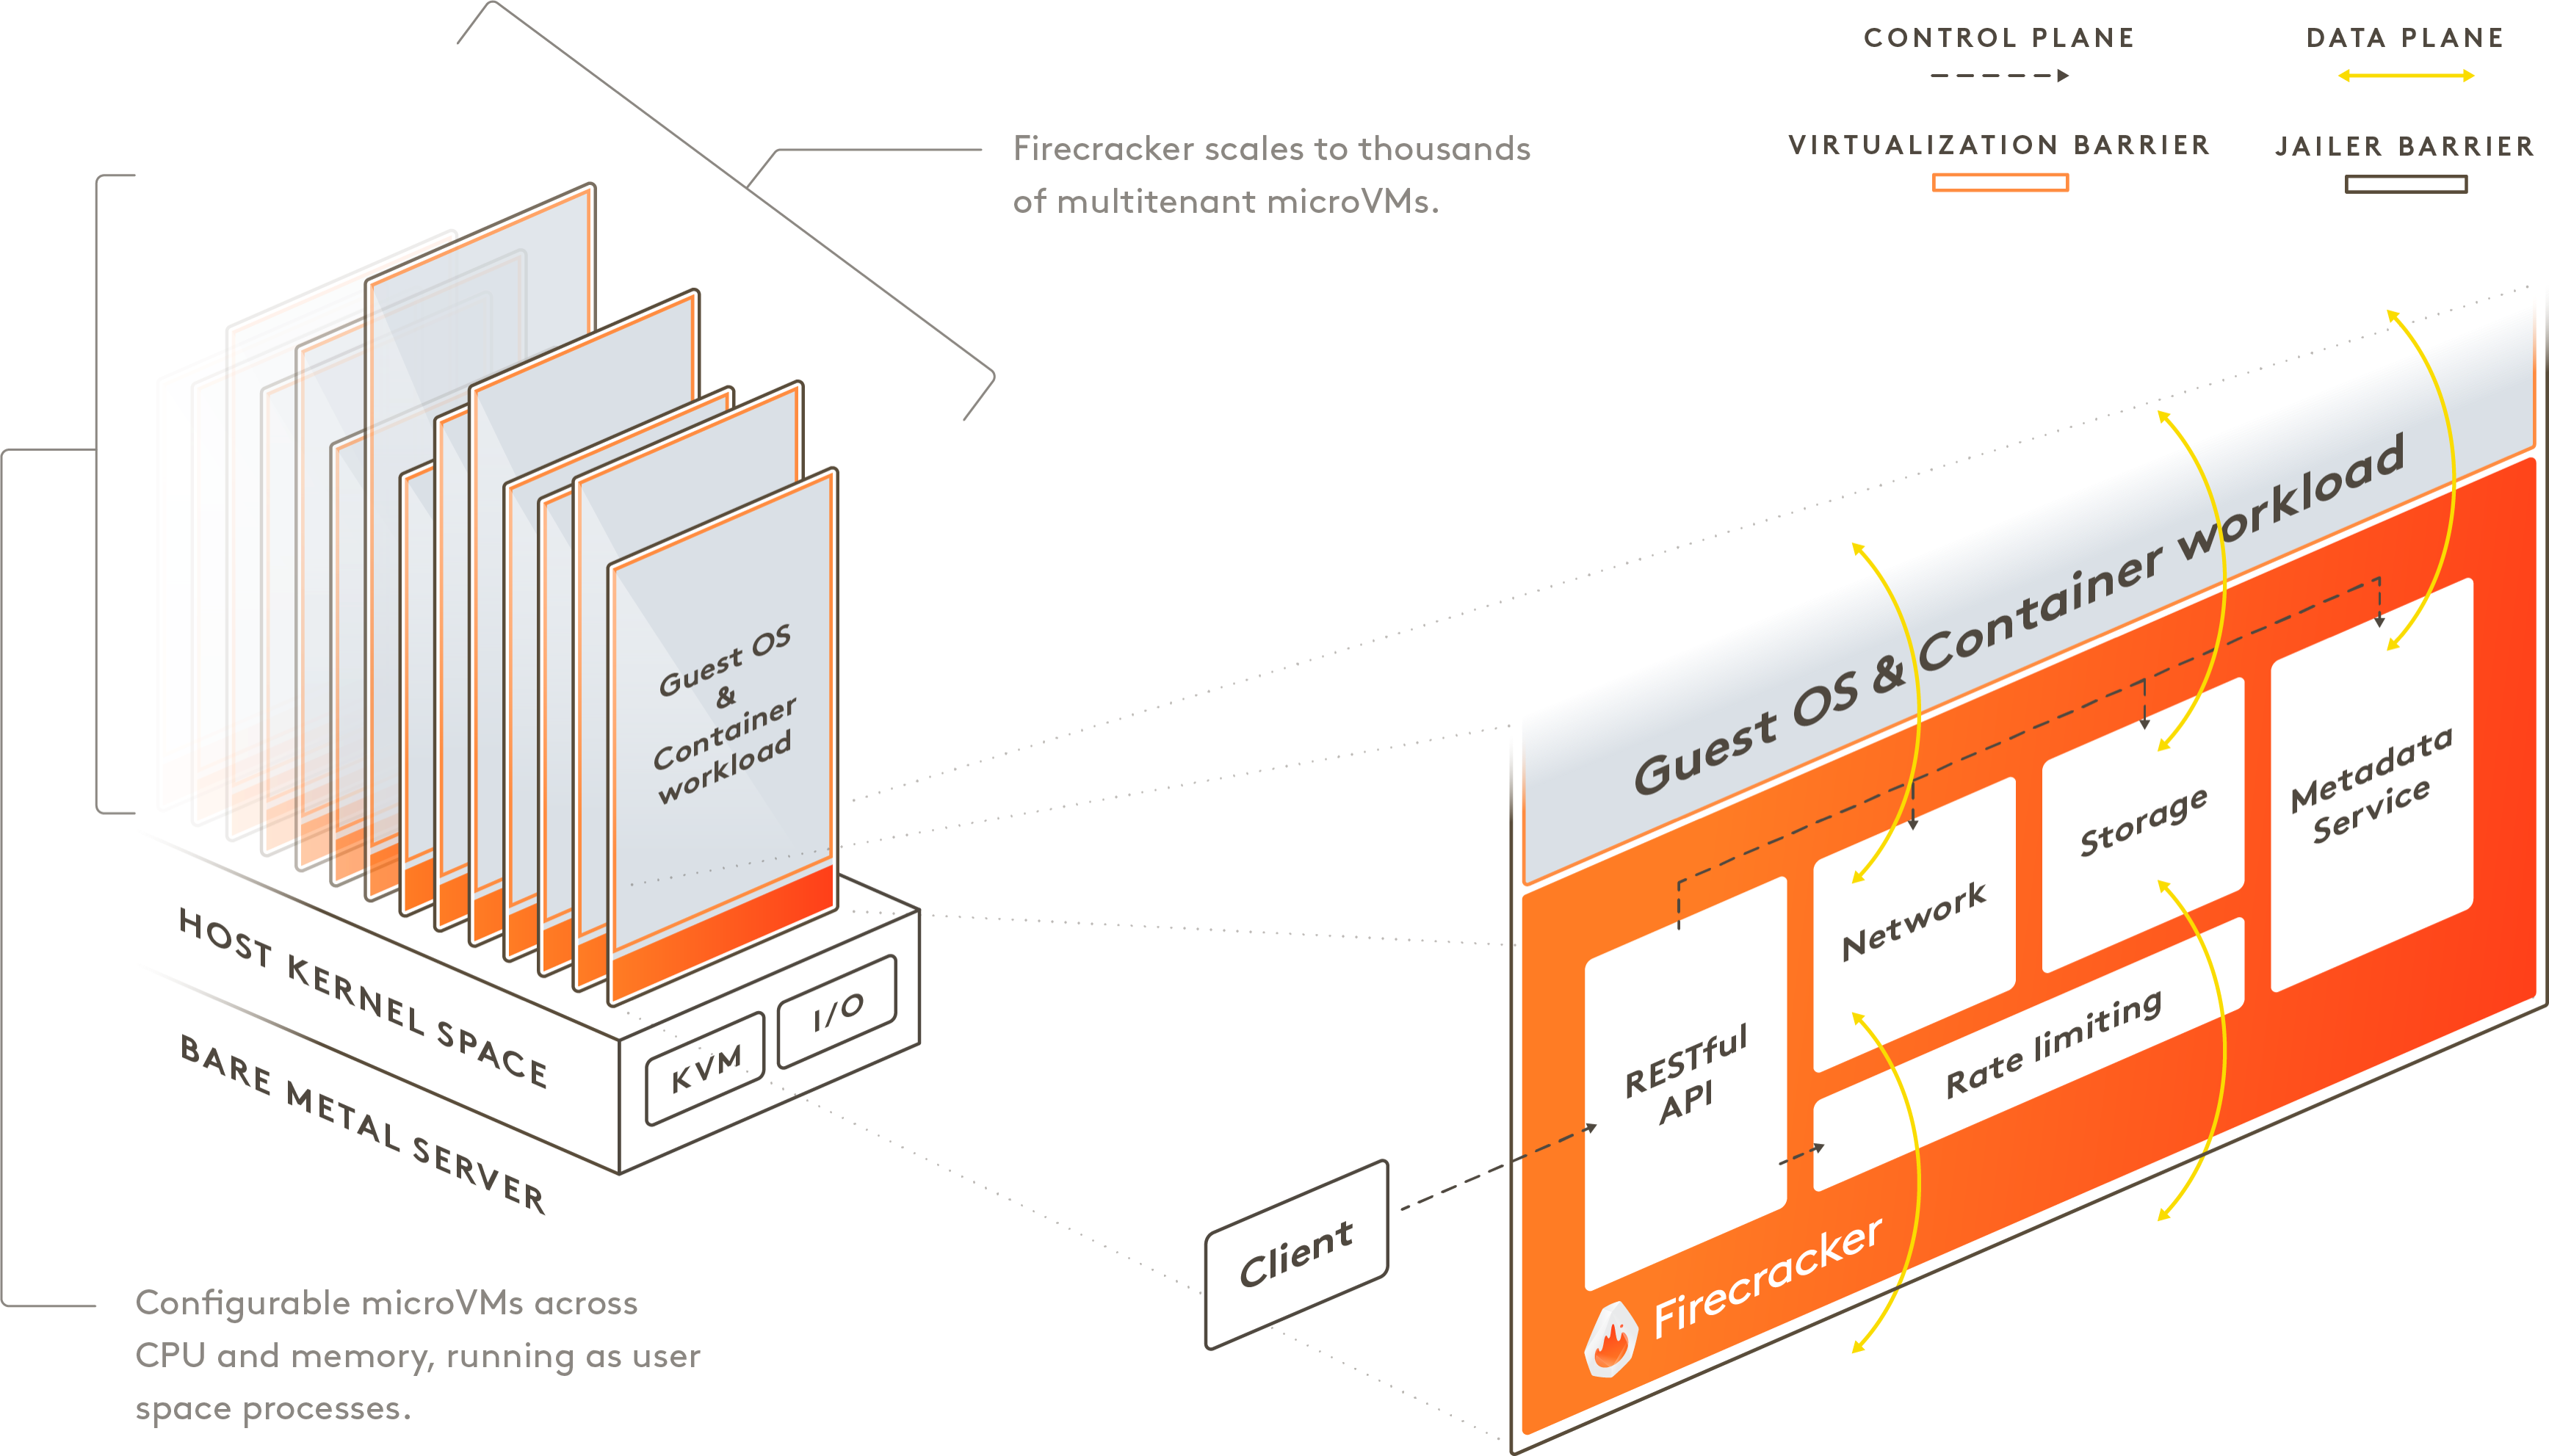
\includegraphics[width=0.7\textwidth]{./2-Basic-Concepts/firecracker-diagram.png}
    \caption{نمایی از ساختار Firecracker}
    \label{fig:firecracker}
\end{figure}

\section{Go Fiber}
زبان استفاده شده در میکروسرویس ها Go می‌باشد که توسط گوگل توسعه داده شده و از فریمورک Fiber استفاده شده که برای ساده تر شدن routing و middleware استفاده شده است.
از دلایل استفاده از Go میتوان به سادگی و سرعت بالا اشاره کرد. همچنین این زبان در مسائل concurrency ابزارهای low-level زیادی در دسترس کاربر قرار می‌دهد.

\section{RabbitMQ}
RabbitMQ یک نرم افزار برای انتقال پیام بین سیستم ها است.
در این پروژه درخواست اجرا کد در صف وارد می‌شود و توسط سرویسی پردازش می‌شود.
دلیل استفاده از event-driven بلاک نشدن درخواست ها است.

مزیت استفاده از RabbitMQ آسنکرون شدن سیستم است. پیام ها و وضعیت اجرای کد پشت یکدیگر بلاک نمی‌شوند.
همچنین سیستم ها از وجود یکدیگر بی خبر هستند و وابستگی شان بهم کم می‌شود. به این معماری loosely-coupled می‌گویند.

\section{PostgreSQL}
دیتابیس اصلی استفاده شده PostgreSQL می‌باشد که از نوع رابطه ای است.
جداول این نرم افزار شامل کاربران و کدها می‌باشد.
دلیل انتخاب PostgreSQL مورد اطمینان بودن و سادگی این پایگاه داده بوده است.
برای ارتباط و کوئری زدن از کتابخانه gorm زبان Go استفاده شده که ORM محبوبی  است.

\section{Next.js}
فریمورک استفاده شده سمت کلاینت Next.js می‌باشد که از کتابخانه React برای رندر روی مرورگر استفاده میکند.
دلیل استفاده از React ساده کردن پیاده سازی رابط کابری توسط هوک ها و کامپوننت محور بودن آن است.

زبان برنامه نویسی سمت کلاینت TypeScript است که به واسطه کامپایلر تبدیل به JavaScript می‌شود.
دلیل استفاده از TypeScript اضافه شدن شی‌گرایی و تایپ در زمان کامپایل است.

\chapter{معماری پروژه}


همانطور که در {\ref{fig:architecture}} می‌بینید این پروژه از معماری میکروسرویس بهره می‌برد.
در ادامه به معرفی سرویس ها می‌پردازیم.


\chapter{معماری پروژه}

همانطور که در {\ref{fig:architecture}} می‌بینید این پروژه از معماری میکروسرویس بهره می‌برد.
در این فصل ابتدا به معرفی کلی هر سرویس و سپس نگاهی دقیق به عملکرد هر سرویس می‌اندازیم.

\begin{figure}[htbp]
    \centering
    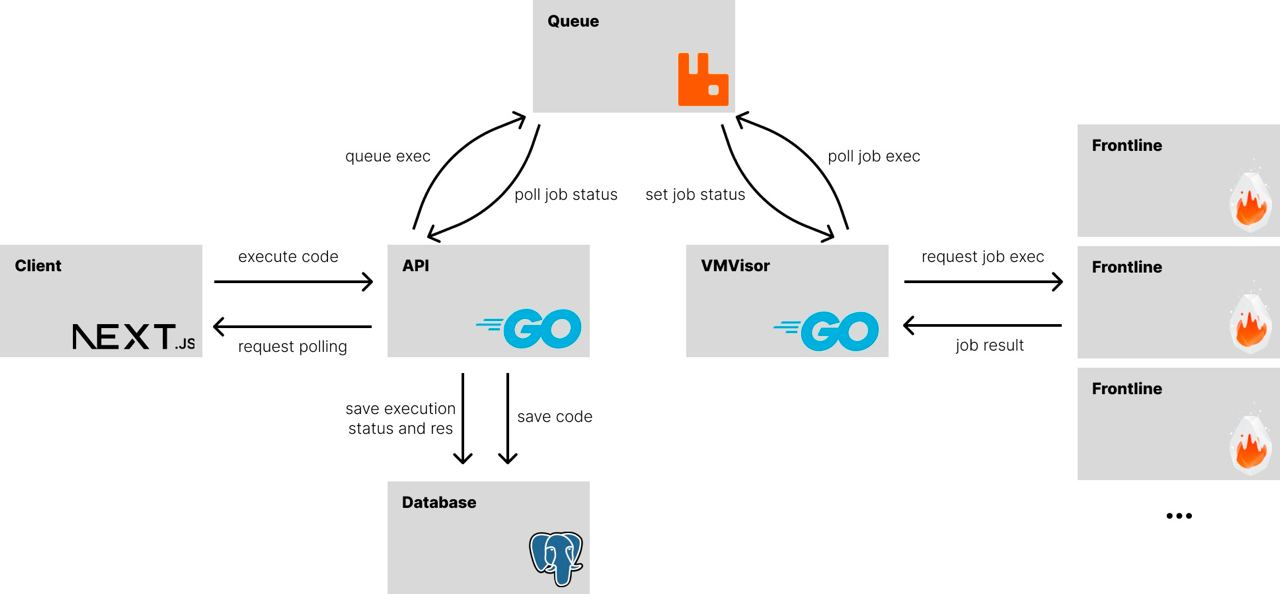
\includegraphics[width=1\textwidth]{./3-Design/design.jpg}
    \caption{معماری پروژه}
    \label{fig:architecture}
\end{figure}

\newpage

همانطور که در شکل و جدول مشاهده می‌کنید پروژه از ۴ سرویس اصلی تشکیل شده است.
درخواست از کلاینت شروع شده پس از طی کردن API و VMVisor به Frontline می‌رسد.
پیش تر اشاره کردیم که Frontline یه Web API است که درون vm در حال اجراست.
Frontline در اصل یک Web API است که با پروسه فرزند کامپایلر زبان های مختلف را فراخوانی کرده و خروجی را بر می‌گرداند.


\begin{table}[hb]
    \centering
    \caption{لیست سرویس ها}
    \label{table:services}
    \begin{tabular}{|c|c|}
        \hline
        سرویس ها  & توضیحات                                                                \\
        \hline

        API       & سرویس REST API است که وظیفه صحبت با دیتابیس و پاسخ به کلاینت را دارد   \\
        \hline

        VMVisor   & مدیریت VM های ساخته و دریافت و تغییر وضعیت درخواست های اجرا روی صف     \\
        \hline

        Frontline & درون هر VM در حال اجراست و توسط پروسه فرزند کامپایلر زبان را صدا می‌زند \\
        \hline


        Client    & کلاینت وطیفه نمایش رابط کاربری و ادیتور را دارد                        \\
        \hline
    \end{tabular}
\end{table}


مهم ترین سرویس این پروژه VMVisor است که وظیفه مدیریت vm ها را بر عهده دارد.
این پروژه از Firecracker استفاده می‌کند و مجموعه ای از vm ها را مدیریت و به آن ها وظیفه ای برای اجرا می‌سپارد.


ارتباط بین API و VMVisor به صورت آستکرون توسط انتقال پیام در صف است.
در RabbitMQ دو صف وجود دارد. صف درخواست اجرا و صف وضعیت اجرا.
در صف درخواست اجرا سرویس API کدی که کلاینت ارسال کرده را روی صف قرار می‌دهد
و VMVisor این درخواست را از صف بر‌می‌دارد.
صف دیگر وضعیت اجرا است که VMVisor خروجی Frontline را روی صف قرار می‌دهد و API به آن گوش می‌دهد و روی پایگاه داده می‌نویسد.

وظیفه API عملیات های CRUD(create read update delete) است و اولین درگاهی است که کلاینت با آن در ارتباط است.
همچنین وظیفه قرار دادن درخواست اجرا در صف و گوش دادن به صف وضعیت اجرا و نوشتن آن روی پایگاه داده را برعهده دارد.
از دیگر وظیفه های این سرویس مدیریت کاربران و پروژه های آن ها است.
این سرویس خود پتانسیل شکسته شدن به میکروسرویس های کوچک تر را دارد ولی در این پروژه این تصمیم گرفته نشده است.

کلاینت هم بخش مهم دیگری است که رابط کاربری سیستم با نرم افزار است. کاربر امکان ساخت پروژه جدید و ویرایش آن در مرورگر را دارد.
رابط کاربری این پروژه در Figma طراحی شده و توسط کتابخانه React دیزاین سیستم طراحی شده و کامپوننت های مختلف در کنار هم قرار گرفته اند.

در ادامه به معرفی دقیق تر هر سرویس و ارتباطش با سایرین می‌پردازیم.

\newpage


\section{API}

همانطور که اشاره کردم بخش API پروژه از زبان Go و فریمورک Fiber استفاده می‌کند.
این پروژه لایه ورودی ما به بخش های داخلی سیستم می‌باشد.

در عکس زیر نمایی از api های موجود در پروژه مشاهده می‌شود.
این api ها در چند دسته مختلف تقسیم بندی شده اند. sandbox برای ساخت یک پروژه جدید و اجرا آن می‌باشد.
بخش auth برای ثبت نام و ورود کاربر است.
بخش user برای دریافت اطلاعات کاربر وارد شده است.
و health برای بررسی liveness و readiness سیستم در نظر گرفته شده است.
وجود این مسیر باعث می‌شود در سیستم های مدیریت کانتینر مانند kubernetes از آمادگی سرویس اطمینان حاصل کرد.

\begin{figure}[hb]
    \centering
    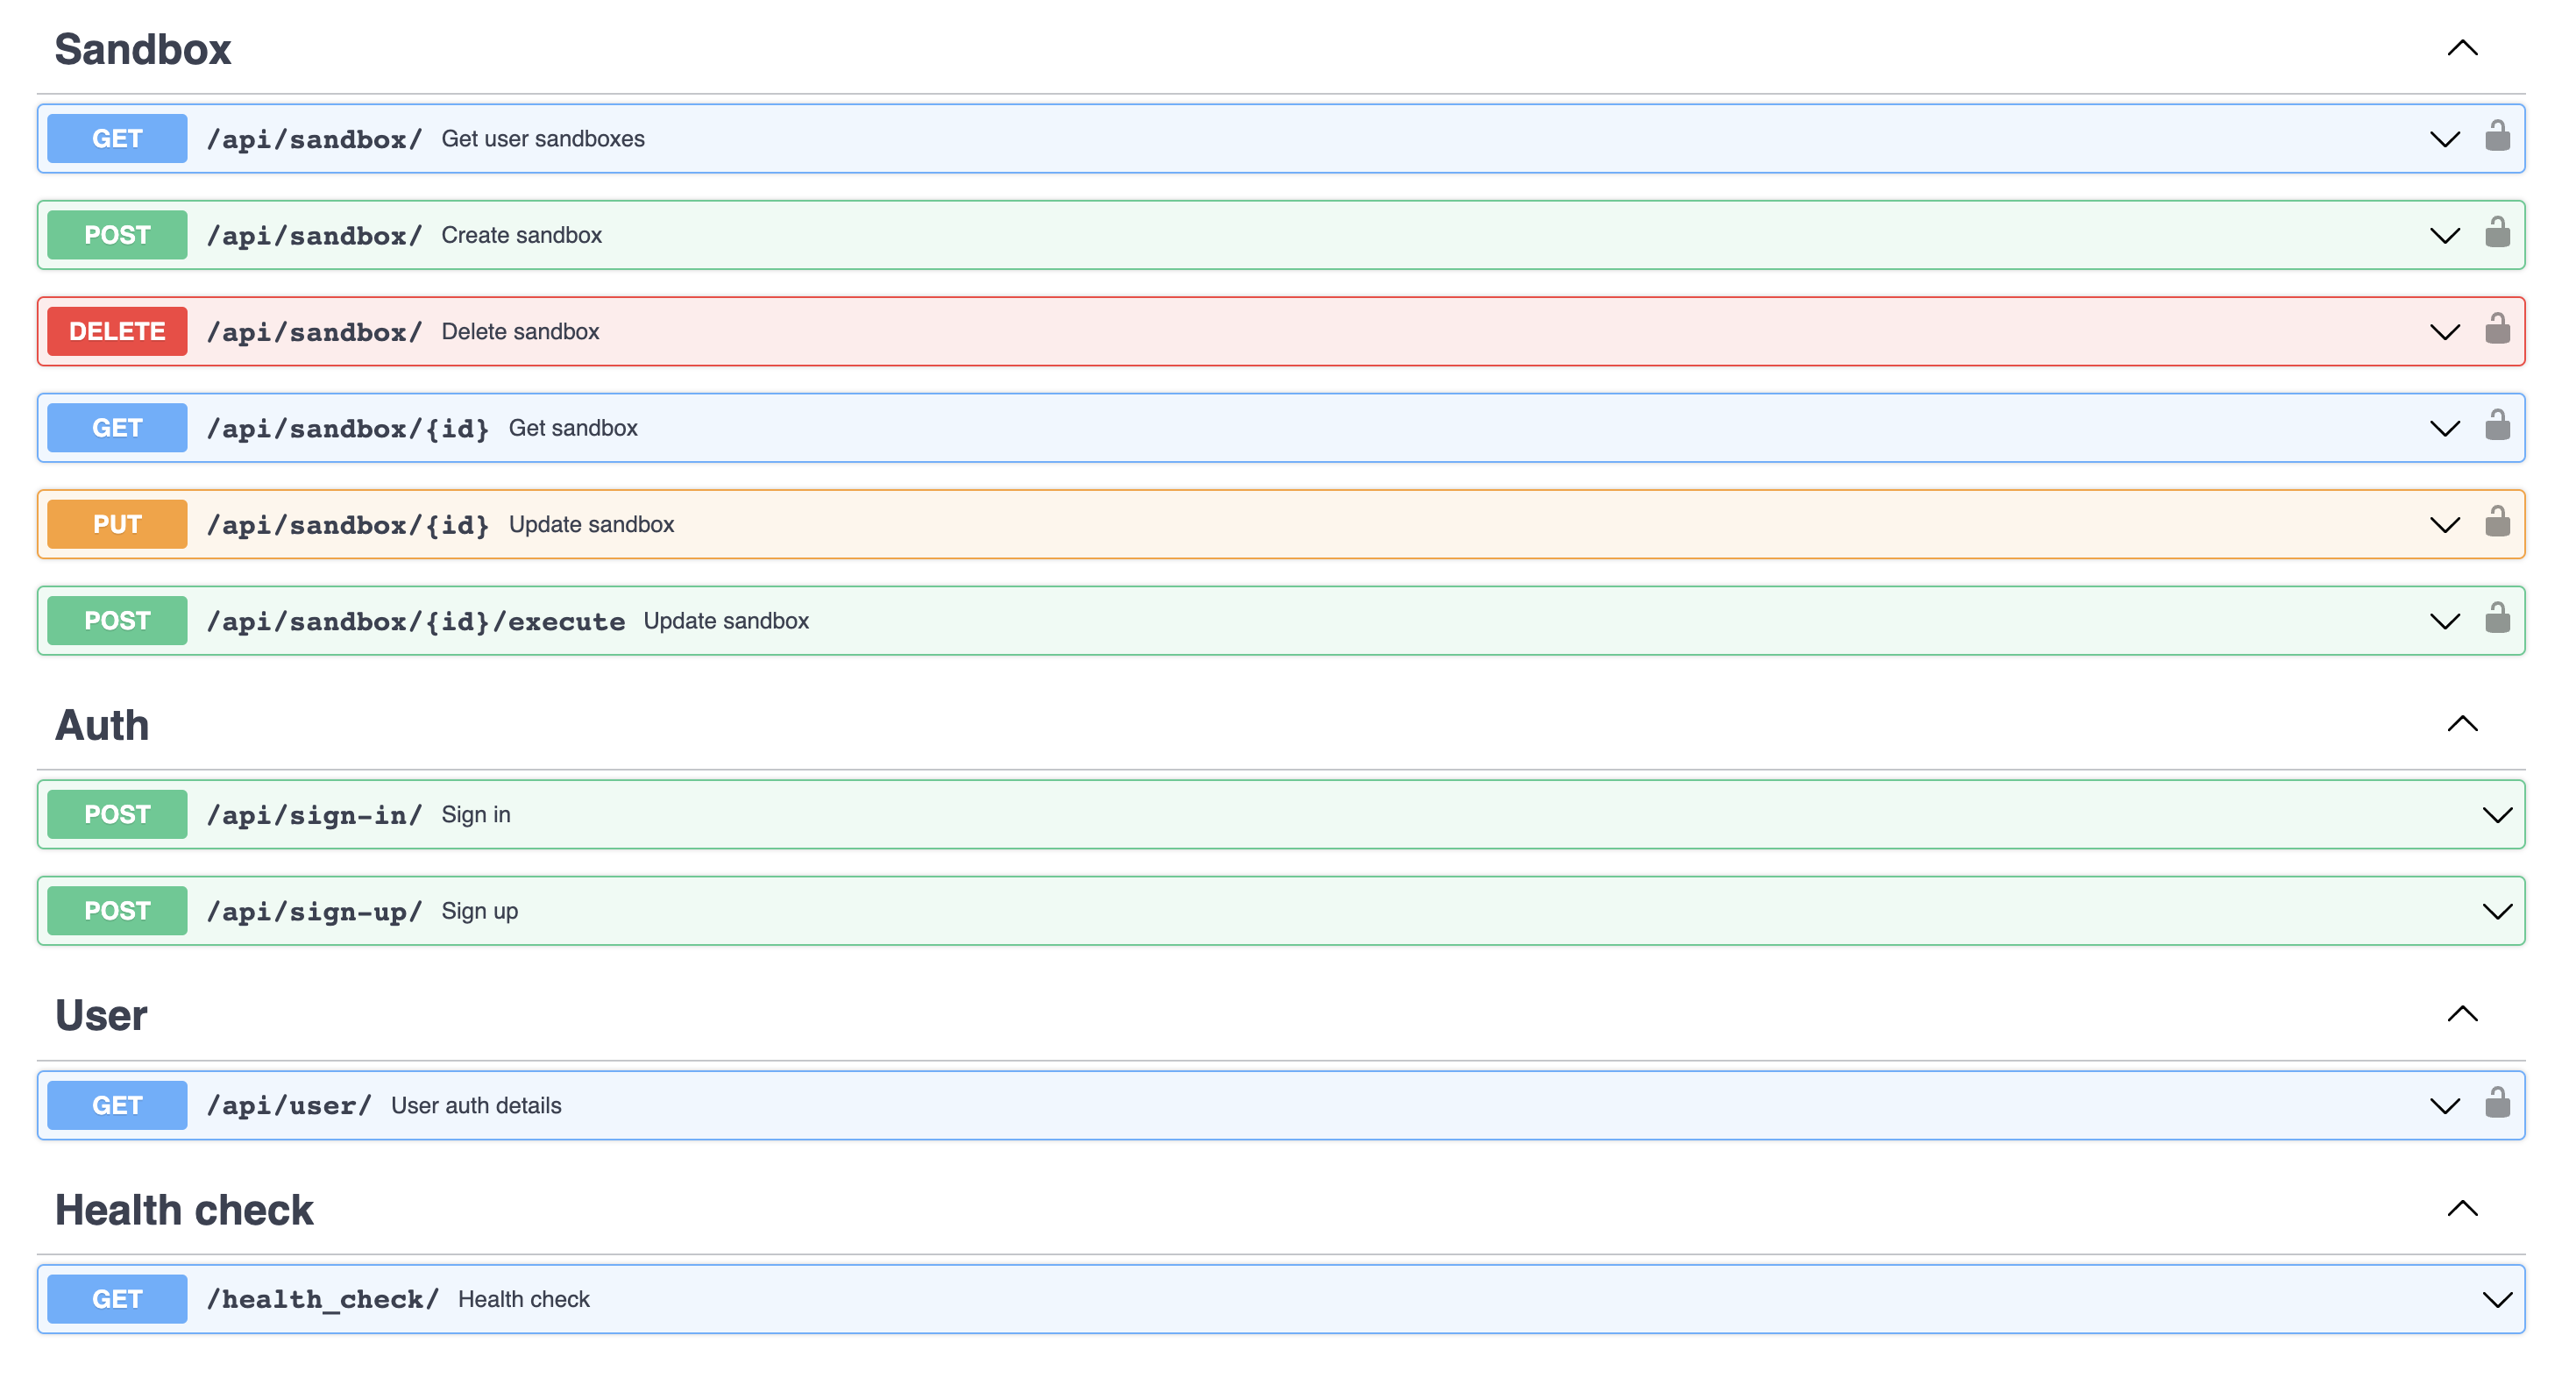
\includegraphics[width=1\textwidth]{./3-Design/swagger.png}
    \caption{لیست API}
    \label{fig:swagger}
\end{figure}


\newpage

\section{VMVisor}
شاید پیچیده ترین سرویس این پروژه VMVisor باشد.
این سرویس چندین وظیفه دارد شامل:

\begin{itemize}
    \item مدیریت و ساختن مجموعه vm
    \item دریافت درخواست اجرا کد از صف
    \item ارتباط با Frontline برای اجرای کد
    \item ارسال تغییر وضعیت کد به صف
\end{itemize}

تعداد مجموعه vm های آماده ۱۰ عدد است. به هر vm یک عدد هسته پردازنده و ۲۵۶ مگابایت حافظه RAM و ۱ گیگابایت فضا اختصاص می‌شود.

ماکسیمم مدت زمان اجرا ۱۰ ثانیه است. پس از آن vm حذف می‌شود.
پس از اجرا یک vm به مجموعه اضافه می‌شود تا تعداد vm های آماده همان ۱۰ عدد بماند.

ارتباط VMVisor با vm از طریق سرویس به نام Frontline است.
Frontline در اصل یک \lr{REST API} است که درون vm در حال اجراست و درخواست را دریافت کرده و خروجی را به VMVisor بر می‌گرداند.
این سرویس سپس وضعیت اجرا را روی صف قرار می‌دهد.


در شکل زیر وضعیت های مختلف اجرا کد را می‌توانید ببینید.

\begin{figure}[htbp]
    \centering
    \caption{وضعیت اجرا کد}
    \label{fig:job-state}
    \begin{tikzpicture}[node distance=2cm]
        \node (received) [startstop] {Received};
        \node (running) [process, right of=received, xshift=2cm] {Running};
        \node (done) [process, right of=running, xshift=2cm] {Done};
        \node (failed_received) [process, below of=received] {Failed};
        \node (failed_running) [process, below of=running] {Failed};

        \draw [arrow] (received) -- (running);
        \draw [arrow] (running) -- (done);
        \draw [arrow] (received) -- (failed_received);
        \draw [arrow] (running) -- (failed_running);
    \end{tikzpicture}
\end{figure}

در ادامه به آخرین تکه پازل یعنی Frontline می‌پردازیم.


\newpage

\section{Frontline}

همانطور که اشاره کردیم Frontline یک \lr{Web API} است که با زبان Go توسعه داده شده.
این سرویس درون vm در حال اجراست و از طریق پردازه فرزند کامپایلر زبان مورد نظر را فراخوانی می‌کند.

این سرویس از طریق openrc که سرویس init برای لینوکس است بلافاصله بعد از بوت vm در حال اجرا قرار می‌گیرد.

درون فایل سیستم هر vm تمام کامپایلرهای مورد نیاز قرار دارد.
این فایل سیستم با دستور dd با فضای یک گیگابایت ساخته شده است
و از طریق docker روی آن نوشته می‌شود.

این پروسه توسط اسکریپتی انجام می‌شود. در این اسکریپت توسط alpine و پکیج منجر آن کامپایلر زبان های مختلف دانلود می‌شود.
فایل سیستم به عنوان volume برای docker اضافه می‌شود و از این طریق امکان نصب این کامپایلر ها روی آن امکان پذیر می‌شود.

هر vm نیاز به گرفتن ip دارد. VMVisor از طریق درخواست HTTP با Frontline در ارتباط است.
برای بحث نتورکینگ از CNI استفاده شده است که از بحث این مقاله خارج است.

درون Frontline دو مسیر اصلی وجود دارد.
health و exec. health برای بررسی آمادگی vm به کار می‌رود.
پیش تر اشاره کردیم که وظیفه VMVisor آماده نگه داشتن ۱۰ vm است.
ساختن vm جدید ممکن است چندین ثانیه طول بکشید. هر ۱۰ ثانیه VMVisor درخواستی به health می‌زند و پس از دریافت ۲۰۰ آن vm را به مجموعه اضافه می‌کند.



\newpage


\section{کلاینت}
همانطور که اشاره کردیم کلاینت این پروژه از Next.js استفاده می‌کند.
طراحی رابط کاربری در محیط Figma انجام شده است.


مراحل پیاده سازی به شرح زیر است:
\begin{enumerate}
    \item دیزاین توکن ها را استخراج و به پروژه اضافه می‌کنیم. مانند رنگ ها، فاصله ها و سایه ها
    \item المنت های دیزاین سیستم رو پیاده سازی می‌کنیم. کامپوننت هایی مانند دکمه، اینپوت و کانتینر
    \item با کنار هم قرار دادن المنت های دیزاین سیستم و کامپونتت های مخصوص هر بخش، صفحه را تکمیل می‌کنیم
    \item مراحل دریافت یا فرستان اطلاعات را انجام می‌دهیم
    \item مرحله ۳ و ۴ را برای هر صفحه تکرار میکنیم
\end{enumerate}

\begin{figure}[htbp]
    \centering
    \begin{subfigure}[b]{0.26\textwidth}
        \centering
        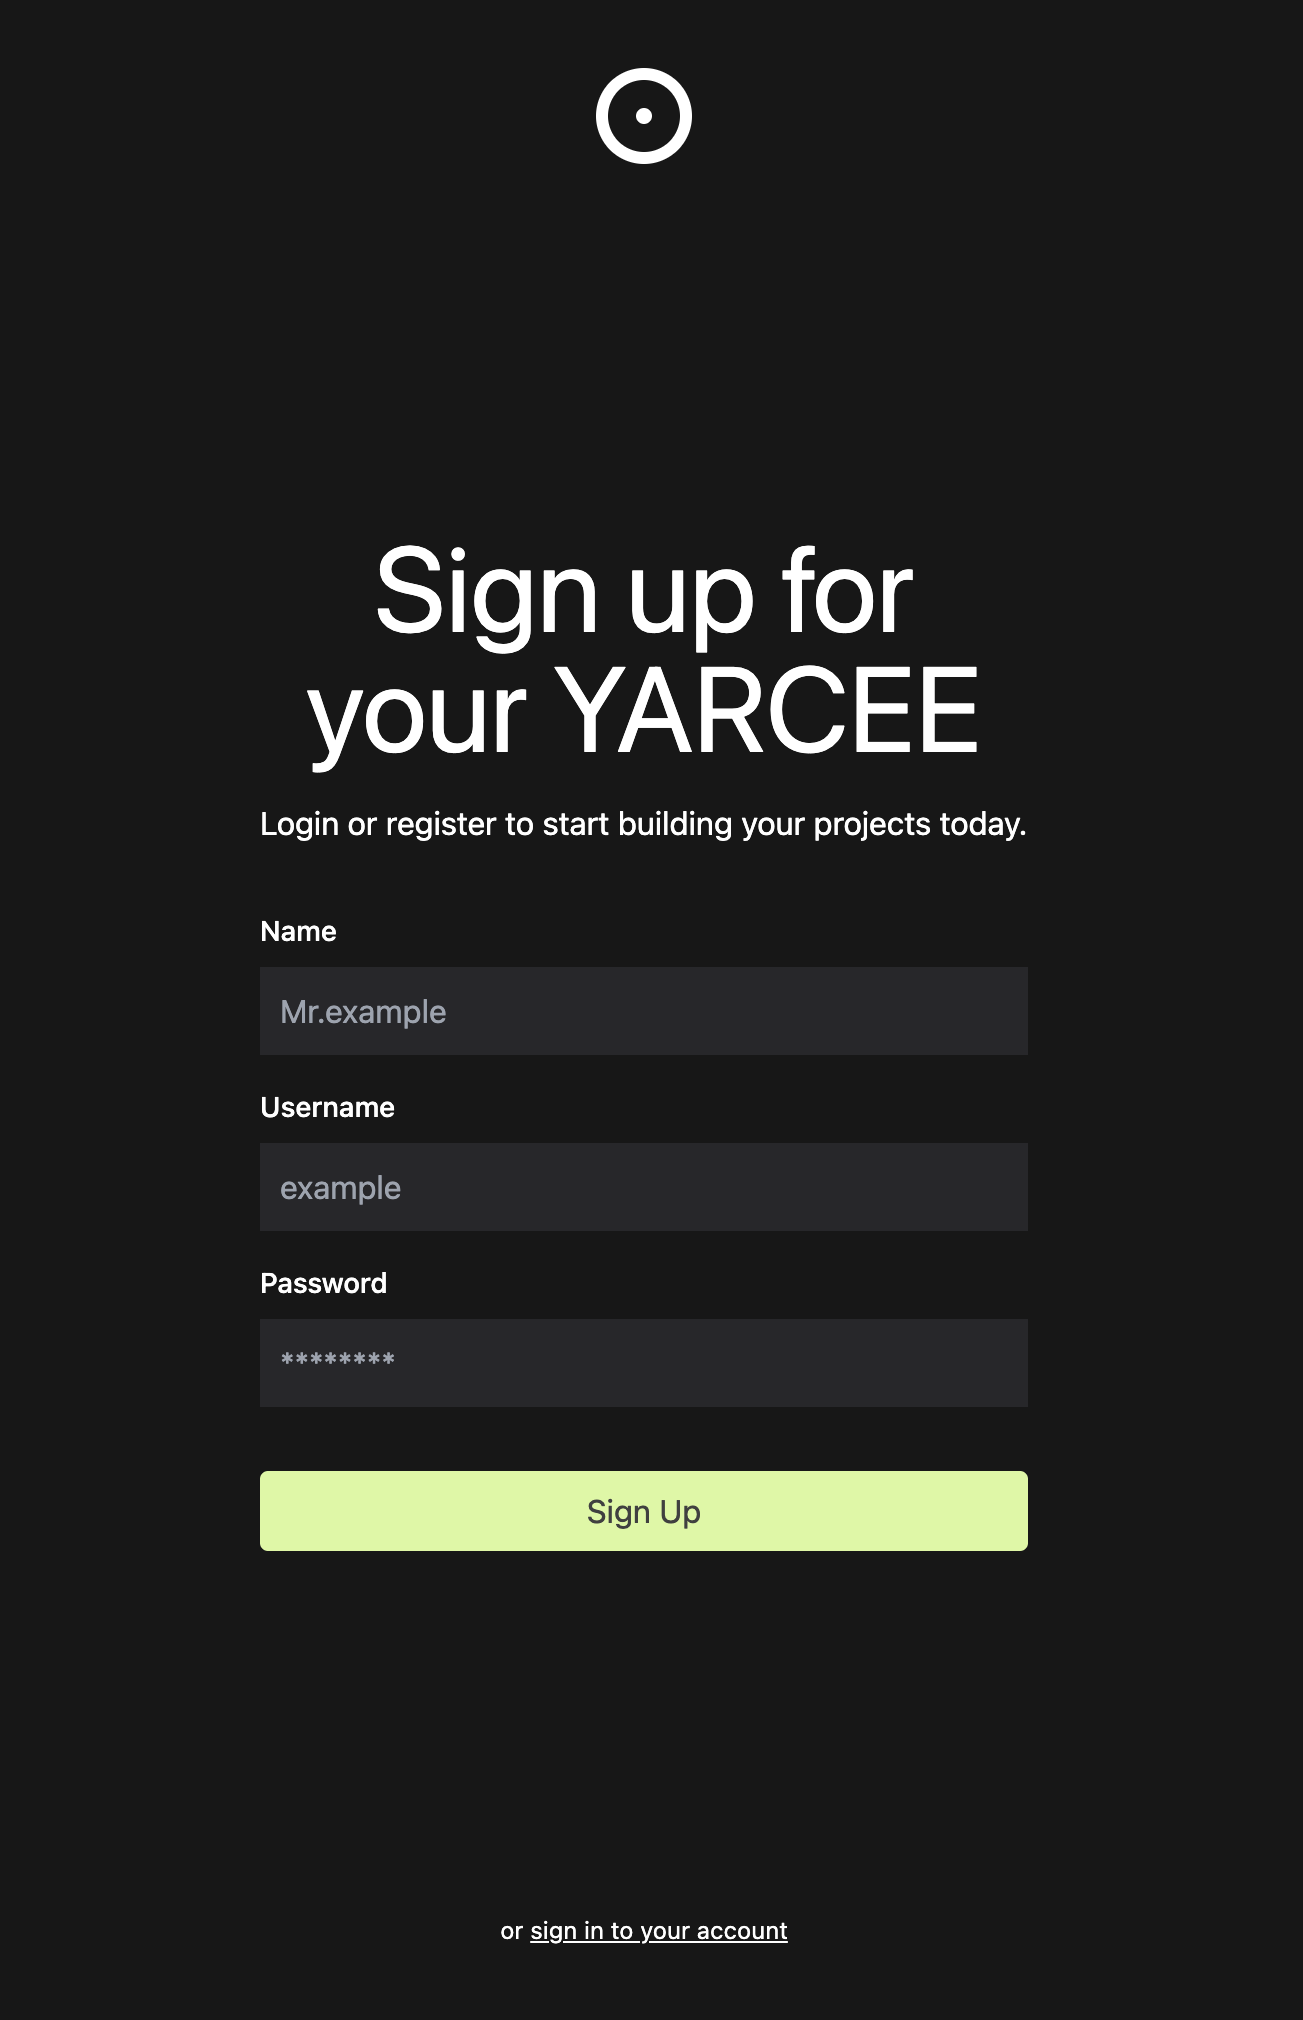
\includegraphics[width=\textwidth]{./3-Design/signup.png}
        \caption{صفحه ثبت نام}
        \label{fig:signup}
    \end{subfigure}
    \hfill
    \begin{subfigure}[b]{0.70\textwidth}
        \centering
        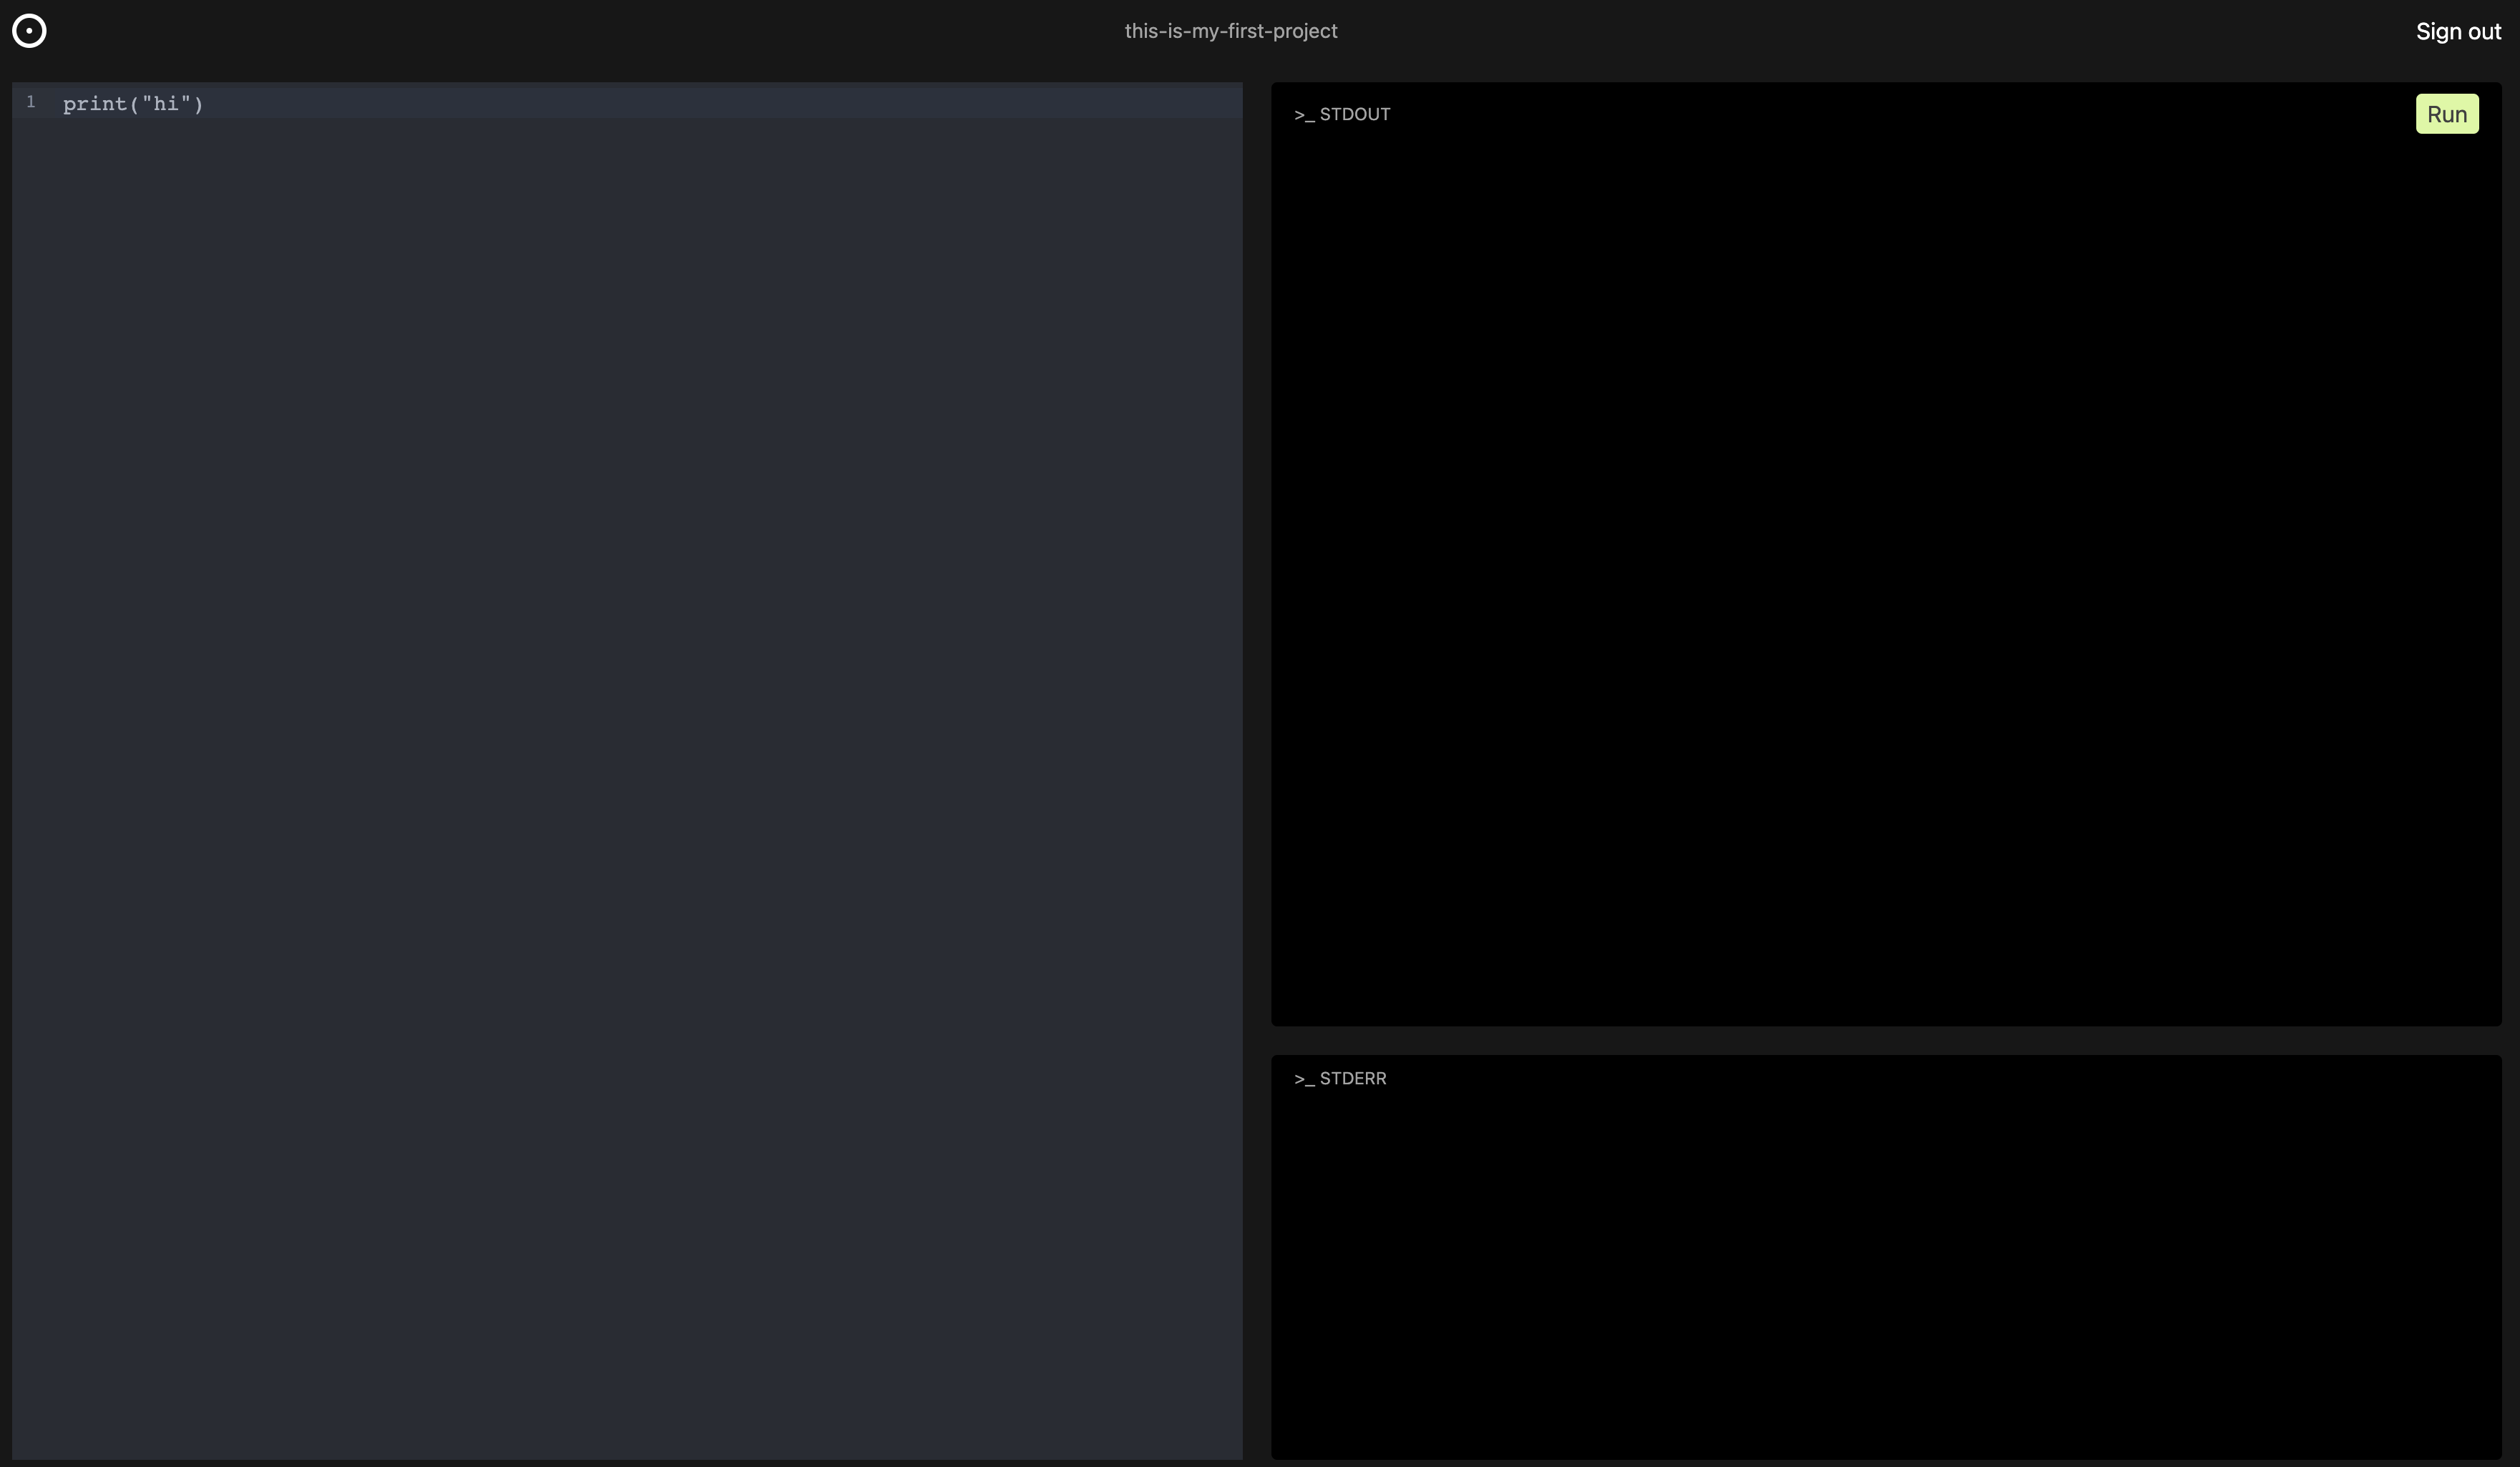
\includegraphics[width=\textwidth]{./3-Design/editor.png}
        \caption{صفحه ادیت کد}
        \label{fig:editor}
    \end{subfigure}

    \caption{طرح برخی از صفحه ها}
\end{figure}

در شکل بالا میتوانید نمونه ای از صفحه های پیاده سازی شده در این پروژه را مشاهده کنید.


\begin{figure}[h]
    \centering
    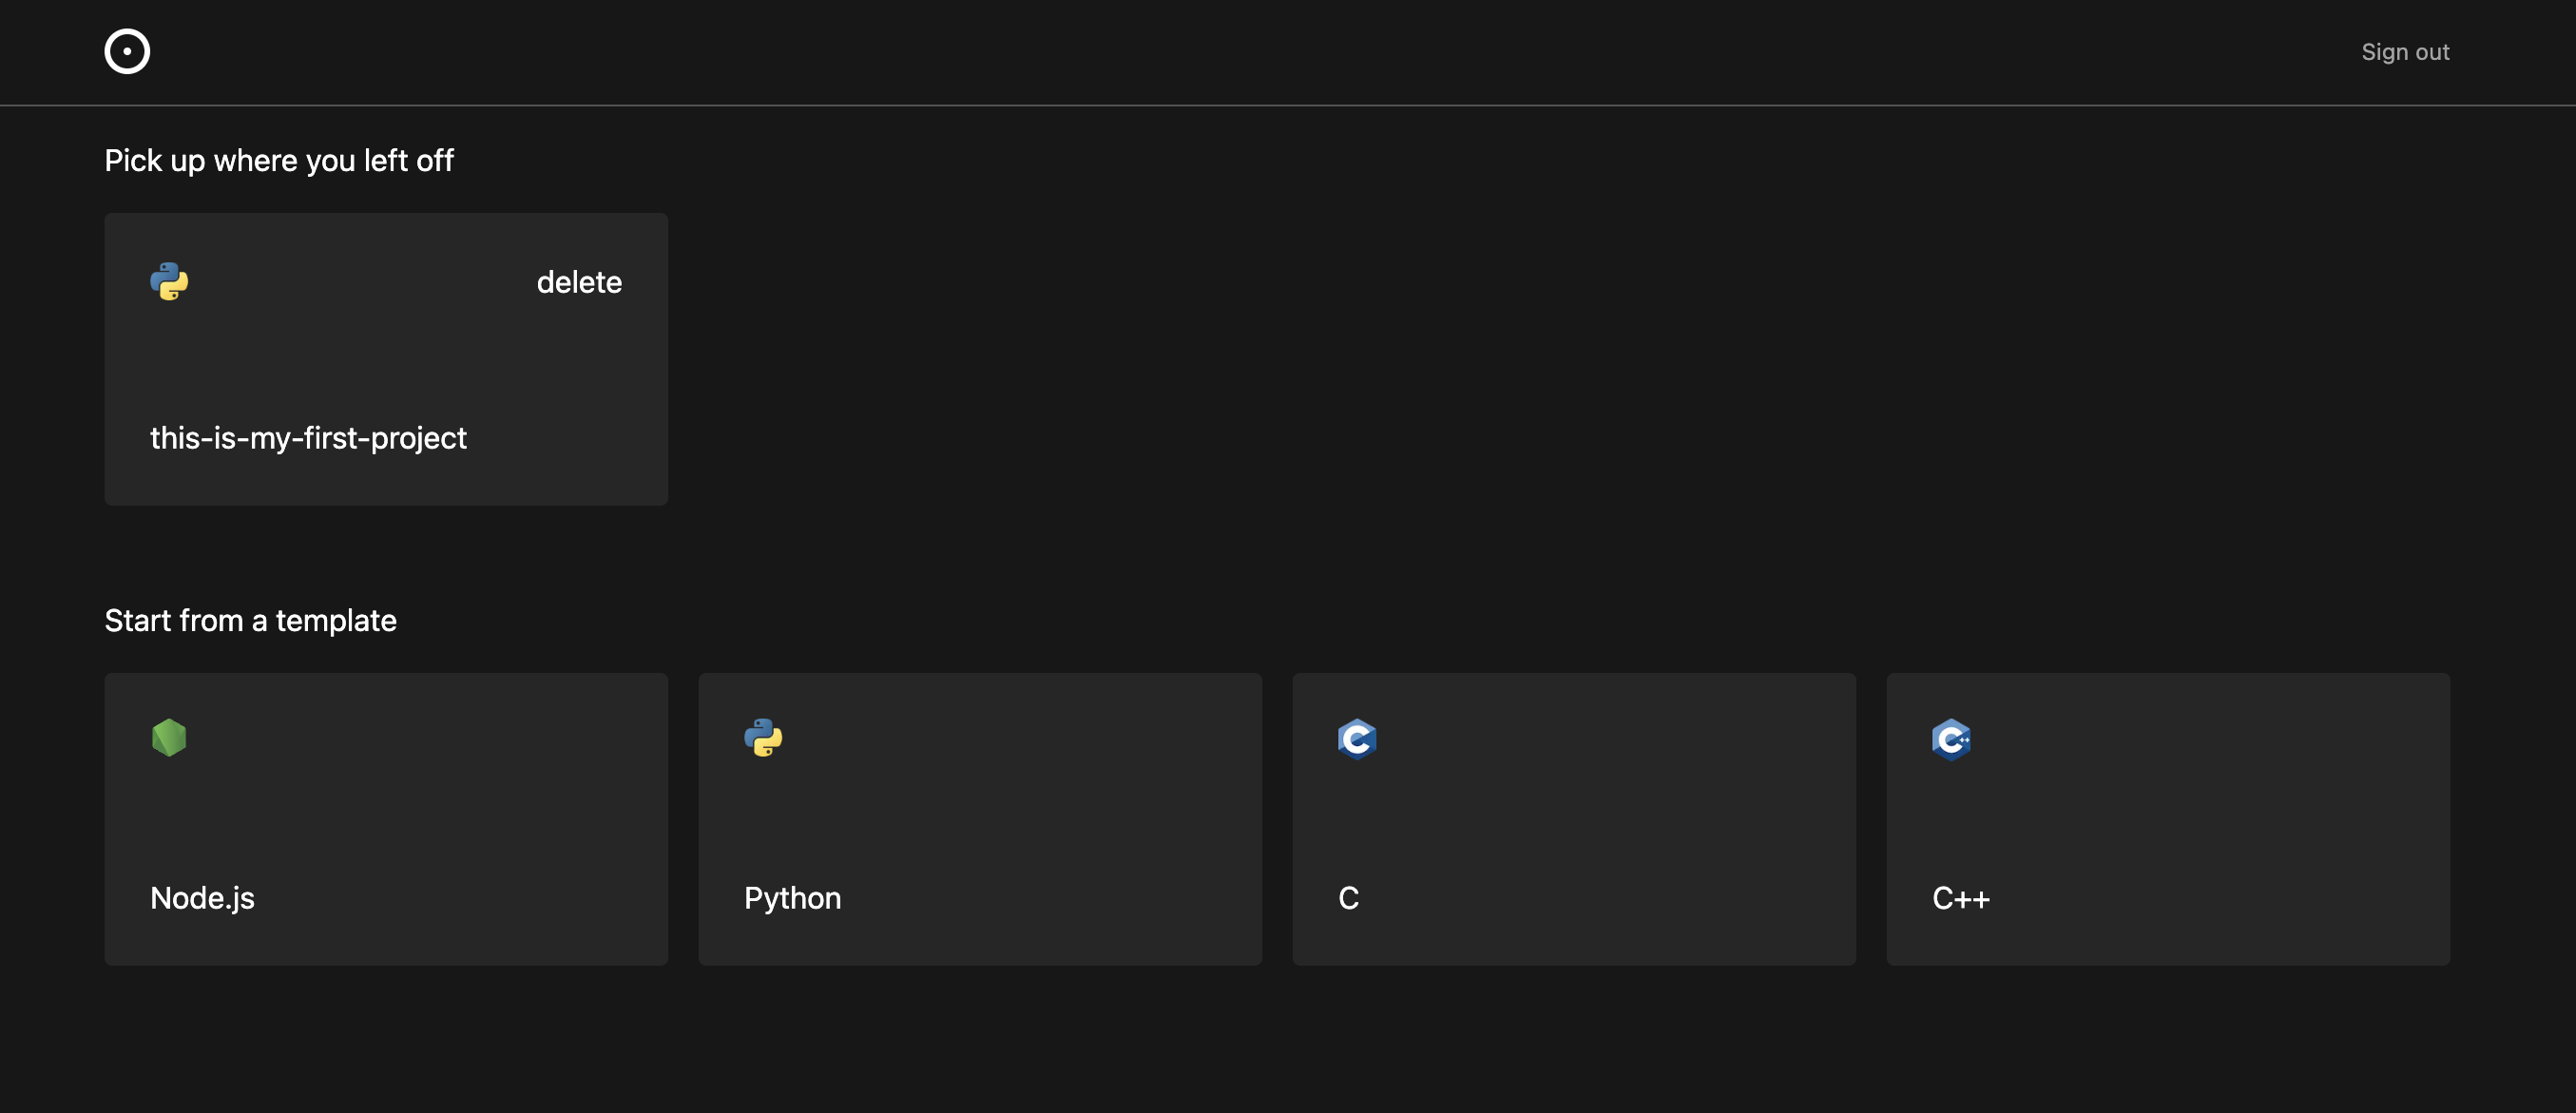
\includegraphics[width=1\textwidth]{./3-Design/projects.png}
    \caption{لیست پروژه ها}
    \label{fig:projects}
\end{figure}

پس ثبت نام و ورود به سایت شما با صفحه داشبورد مواجه می‌شوید. در این صفحه می‌توانید به ادامه ویرایش پروژه قبلی خود بپردازید یا توسط قالب های از پیش تعیین شده پروژه جدیدی شروع کنید.
اضافه کردن اکثر زبان های برنامه نویسی ممکن است ولی در حال حاضر از Python، Node.js، C و C++ پشتیبانی می‌شود.

اضافه کردن زبان جدید به سادگی امکان پذیر است که در ادامه در بخش Frontline به آن می‌پردازیم.


\chapter{ویژگی از دید کاربر}

\section{کلاینت}
همانطور که اشاره کردیم کلاینت این پروژه از Next.js استفاده می‌کند.
طراحی رابط کاربری در محیط Figma انجام شده است.


مراحل پیاده سازی به شرح زیر است:
\begin{enumerate}
    \item دیزاین توکن ها را استخراج و به پروژه اضافه می‌کنیم. مانند رنگ ها، فاصله ها و سایه ها
    \item المنت های دیزاین سیستم رو پیاده سازی می‌کنیم. کامپوننت هایی مانند دکمه، اینپوت و کانتینر
    \item با کنار هم قرار دادن المنت های دیزاین سیستم و کامپونتت های مخصوص هر بخش، صفحه را تکمیل می‌کنیم
    \item مراحل دریافت یا فرستان اطلاعات را انجام می‌دهیم
    \item مرحله ۳ و ۴ را برای هر صفحه تکرار میکنیم
\end{enumerate}

\newpage

\begin{figure}[htbp]
    \centering
    \begin{subfigure}[b]{0.26\textwidth}
        \centering
        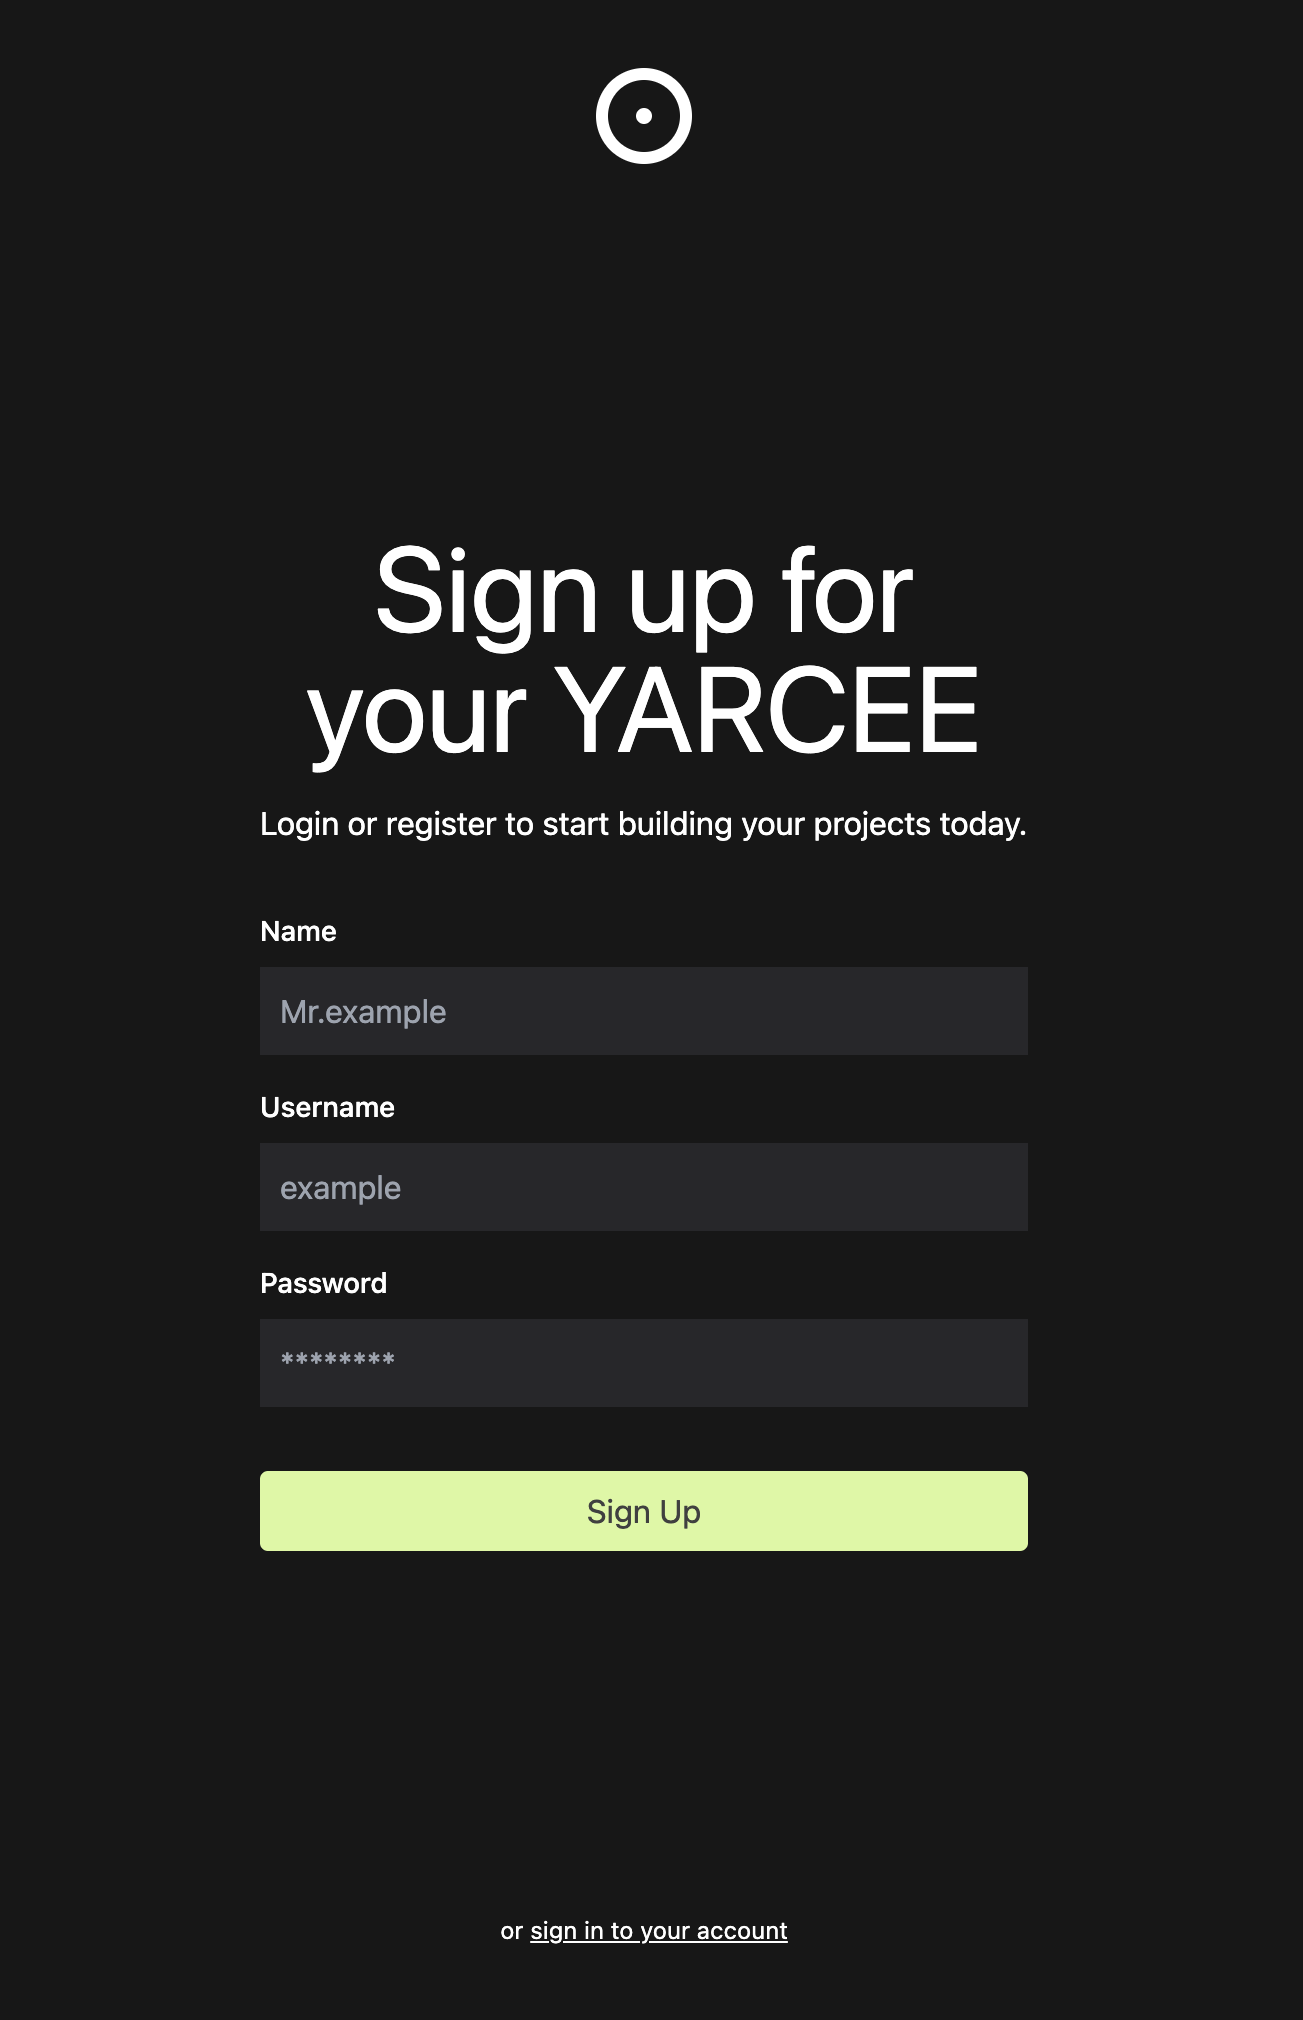
\includegraphics[width=\textwidth]{./3-Design/signup.png}
        \caption{صفحه ثبت نام}
        \label{fig:signup}
    \end{subfigure}
    \hfill
    \begin{subfigure}[b]{0.70\textwidth}
        \centering
        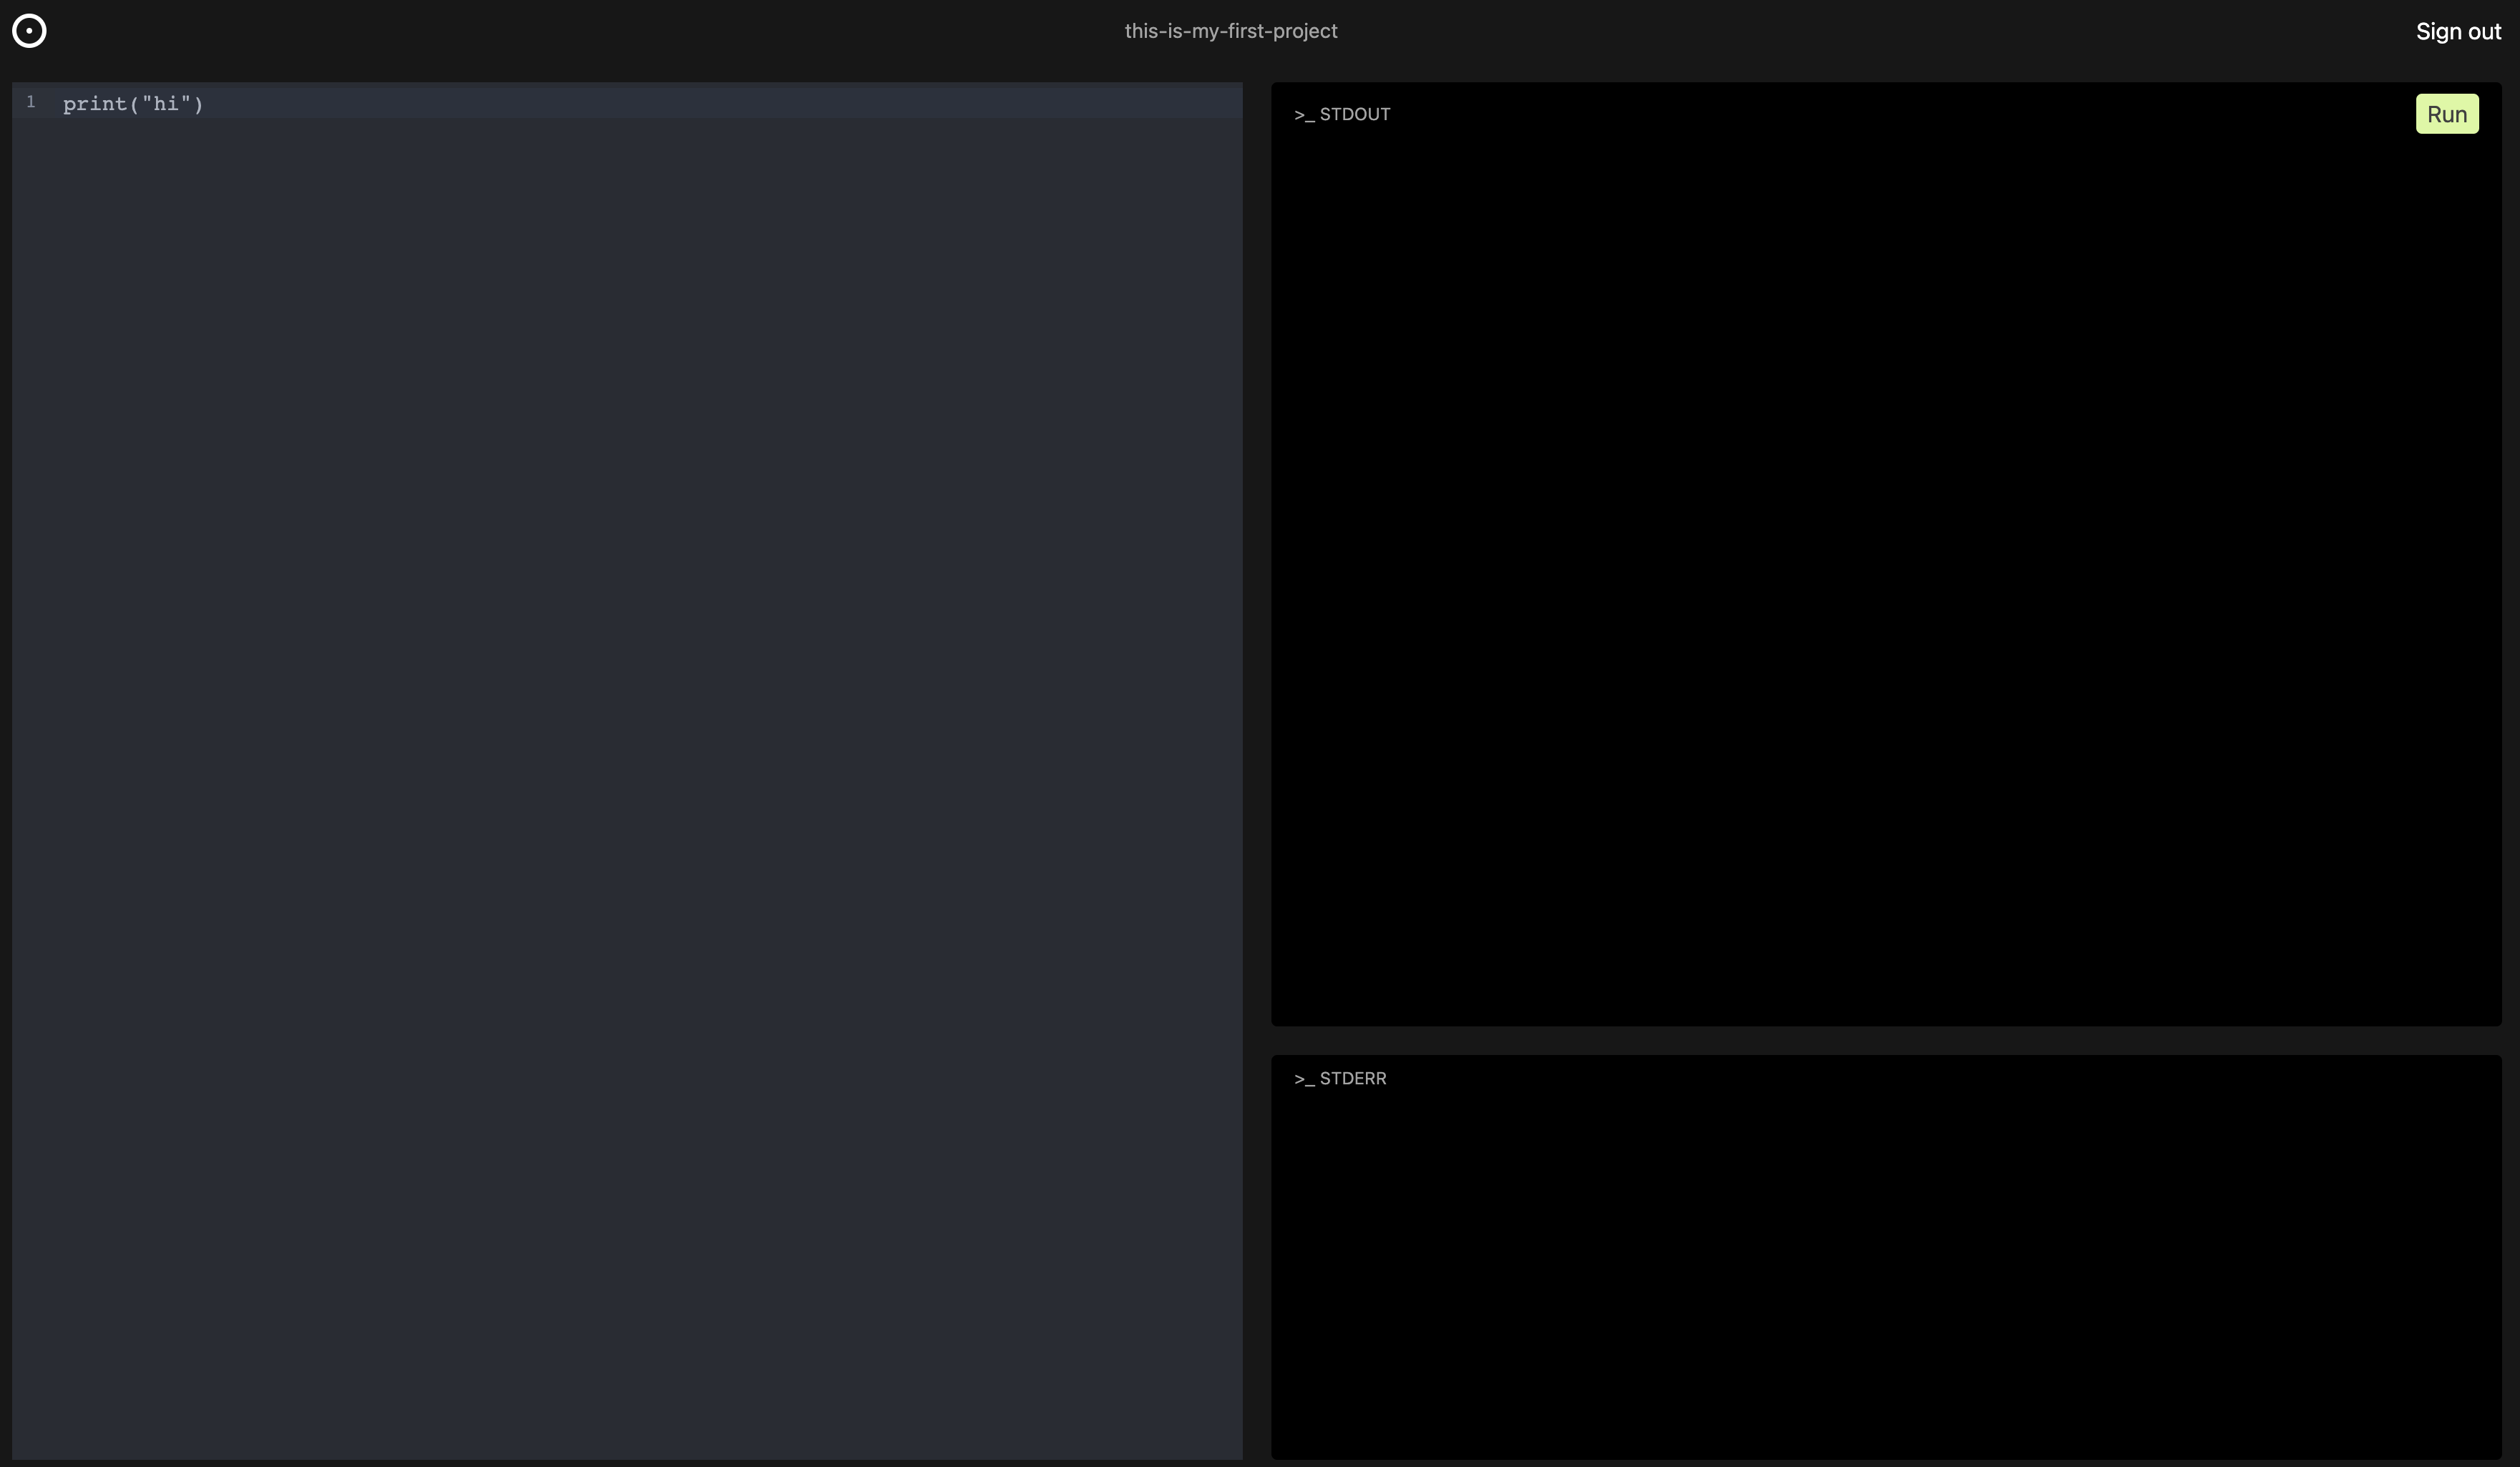
\includegraphics[width=\textwidth]{./3-Design/editor.png}
        \caption{صفحه ادیت کد}
        \label{fig:editor}
    \end{subfigure}

    \caption{طرح برخی از صفحه ها}
\end{figure}

در شکل بالا میتوانید نمونه ای از صفحه های پیاده سازی شده در این پروژه را مشاهده کنید.


\begin{figure}[h]
    \centering
    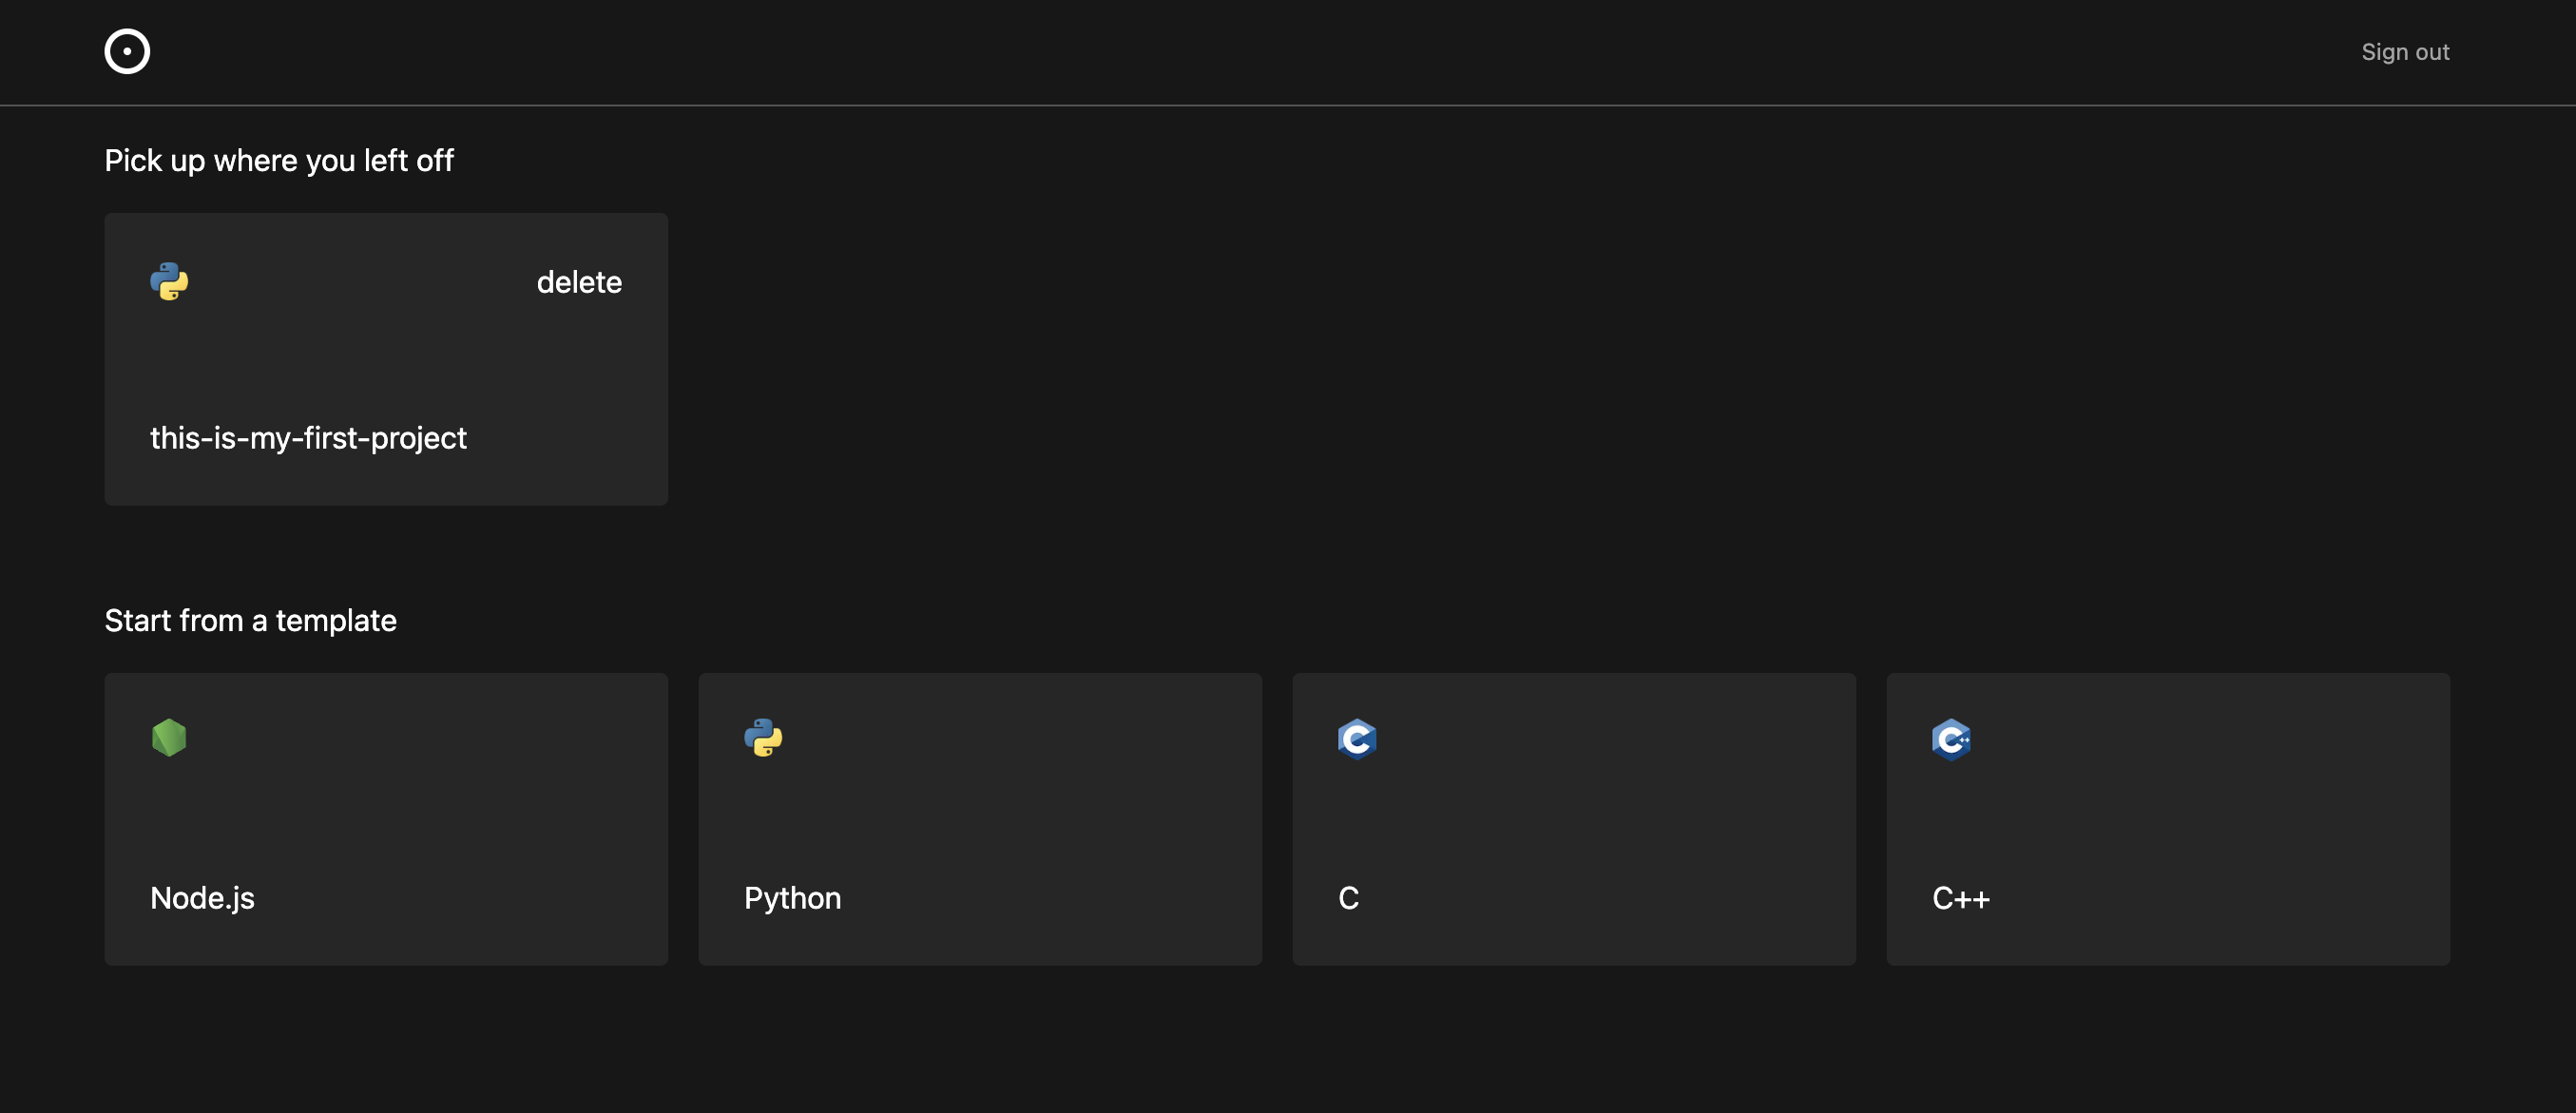
\includegraphics[width=1\textwidth]{./3-Design/projects.png}
    \caption{لیست پروژه ها}
    \label{fig:projects}
\end{figure}

پس ثبت نام و ورود به سایت شما با صفحه داشبورد مواجه می‌شوید. در این صفحه می‌توانید به ادامه ویرایش پروژه قبلی خود بپردازید یا توسط قالب های از پیش تعیین شده پروژه جدیدی شروع کنید.
اضافه کردن اکثر زبان های برنامه نویسی ممکن است ولی در حال حاضر از Python، Node.js، C و C++ پشتیبانی می‌شود.

\chapter{نتیجه گیری و کارهای آتی}



\bibliographystyle{unsrt-fa}
\bibliography{6-Bibliography/References.bib}


%------------------------------------------------------------------------
%	BACK MATTER
%------------------------------------------------------------------------
\backmatter \pagestyle{empty} \pagenumbering{roman}
% Abstract in Latin.
\begin{ParsaAbstractLatin}
    YARCEE(Yet Another Remote Code Execution Engine) is a code running service
    that relies on Firecracker to spawn microVMs and execute the code over HTTP.


    \bigskip\noindent
    \textbf{Keyword:} Remote code execution - MicroVM - VMM
\end{ParsaAbstractLatin}
\clearpage


% Titlepage in English
\titlepageLatin


\end{document}.